\chapter{THÍ NGHIỆM VÀ ĐÁNH GIÁ}\label{chapter:experience}
\vspace{-0.5cm}
\noindent\textit{Trong phần này nhóm sẽ trình bày các thí nghiệm về việc huấn luyện mô hình dựa trên những thay đổi về kiến trúc mô hình, các siêu tham số mô hình, hàm lỗi, dữ liệu huấn luyện ... để đánh giá các ưu nhược điểm đang gặp phải hiện tại đối với việc phân đoạn gan và mạch máu.}\par

\section{Tổng quan}
\subsection{Môi trường thí nghiệm}
\subsubsection{Thông tin phần cứng}
Huấn luyện mạng học sâu với lượng lớn dữ liệu đòi hỏi sức mạnh tính toán cao để công tác huấn luyện diễn ra nhanh chóng và hiệu quả. Để đáp ứng yêu cầu đó, nhóm đã sử dụng hệ thống máy tính hiệu năng cao (HPCC) do GVLab cung cấp. Ngoài ra, nhóm cũng sử dụng Google Colab pro để có thể huấn luyện song song nhiều mô hình.\par

\begin{table}[H]
\centering
\begin{tabular}{@{}ccl@{}}
\toprule
\textbf{STT}       & \textbf{Nguồn cung cấp}       & \multicolumn{1}{c}{\textbf{Cấu hình}}                                             \\ \midrule
\multirow{2}{*}{1} & \multirow{2}{*}{GVLab} & \begin{tabular}[c]{@{}l@{}}GPU: NVIDIA Tesla V100 32GB\\ RAM: 126 GB\end{tabular} \\ \cmidrule(l){3-3} 
                   &                        & \begin{tabular}[c]{@{}l@{}}GPU: NVIDIA Tesla P100 16GB\\ RAM: 126 GB\end{tabular} \\ \midrule
2                  & Google Colab Pro       & \begin{tabular}[c]{@{}l@{}}GPU: NVIDIA Tesla P100 16GB\\ RAM: 12 GB\end{tabular}  \\ \bottomrule
\end{tabular}
\caption{Thông tin phần cứng}
\label{tab:hardware}
\end{table}

\subsubsection*{Ngôn ngữ và framework}
\begin{itemize}[topsep=0pt]
    \item Ngôn ngữ: Python 3.6.9
    \item Framework: PyTorch 1.6.0+cu101
\end{itemize}

\subsection{Phương pháp đánh giá}
Đối với bài toán này, các độ đo được sử dụng để đánh giá mô hình là: Dice, Recall, VOE và VD. Thông tin chi tiết về các độ đo này đã được trình bày ở phần \ref{evaluation-methods}

\section{Thí nghiệm mô hình Unet}

%%%%%%%%%%%%%%%%%%%%%%%%% Mau %%%%%%%%%%%%%%%%%%%%%%%%%%%%%%%%%
\subsection{Thí nghiệm cho đối tượng mạch máu}
\subsubsection{Thí nghiệm về độ sâu của mô hình Unet3D}
Bởi vì sự khác nhau về kích thước giữa các đối tượng (mạch máu, gan) nên việc lựa chọn độ sâu của mô hình đóng phần quan trọng bởi đặc tính của các lớp tích chập và lớp gộp. Nếu mô hình đi càng sâu thì thông tin toàn cục sẽ được chú ý nhiều hơn là thông tin cục bộ, điều này có thể khiến cho mô hình tệ hơn như đã đề cập ở \ref{sec:Unet3D}. 

Nhóm tiến hành huấn luyện mạng Unet3D với các độ sâu khác nhau để tìm được độ sâu (số tầng) phù hợp với mô hình. Các thí nghiệm đều sử dụng hàm đánh giá mất mát: Focal loss với hệ số $\gamma=2$ và $\alpha=0.8$. Kết quả được tính dựa trên trung bình từng hệ số đánh giá cho từng bộ ảnh trong tập kiểm tra. Kết quả tốt nhất thu được trên từng thí nghiệm như sau:

\begin{table}[H]
\centering
\begin{tabular}{c|c|c|c|c}
\Xhline{3\arrayrulewidth}
\multirow{2}{*}{\textbf{Mô hình}} & \multirow{2}{*}{\textbf{Độ sâu}} & \multicolumn{2}{c|}{\textbf{Tập kiểm tra}} & \multirow{2}{*}{\textbf{Số lượng tham số}} \\ 
\cline{3-4} 
&       &\textbf{Dice}       & \textbf{Recall}    &                 \\ \hline
Unet3D  & 3 & 51.58               & 51.33              & 5.420.737       \\ \hline
Unet3D  & 4 & \textbf{55.33}      & 59.06              & 22.399.425      \\ \hline
Unet3D  & 5 & 36.04               & \textbf{65.13}     & 90.304.449      \\

\Xhline{3\arrayrulewidth}
\end{tabular}
\caption{Kết quả thí nghiệm về độ sâu mô hình Unet3D}
\end{table}

Có thể thấy mô hình Unet3D 4 tầng đạt được kết quả khả quan hơn so với độ sâu 3 và 5. Kết quả này có sự khác biệt với mô hình gan bởi vì gan có kích thước lớn hơn máu rất nhiều do đó gan cần mô hình có độ sâu sâu hơn để có được vùng receptive field (vùng mà nơ ron nhìn thấy) rộng hơn để phân biệt được đó có phải là bộ phân gan hay không. Từ thí nghiệm này, nhóm sẽ chọn mô hình Unet3D 4 tầng làm mô hình chính để thực hiện biến đổi cho các thí nghiệm sau.

\subsubsection{So sánh giữa mô hình Unet2D và mô hình Unet3D} \label{exp:2dvs3d}
Để đánh giá được độ hiệu quả của việc phân tích thông tin dưới dạng 3 chiều, nhóm đã tiến hành huấn luyện mạng Unet2D với các thông số giống mạng 3D như mục trên để tiến hành đánh giá. Kiến trúc mạng chỉ được thay đổi các lớp tích chập và lớp gộp từ 3D thành 2D. Và kết quả thí nghiệm như sau:

\begin{table}[H]
    \centering
    \begin{tabular}{c|c|c c| c}
    \Xhline{3\arrayrulewidth}
    \multirow{2}{*}{\textbf{Mô hình}} & \multirow{2}{*}{\textbf{Độ sâu}} & \multicolumn{2}{c|}{\textbf{Tập kiểm tra}} & \multirow{2}{*}{\textbf{Số lượng tham số}} \\ 
    \cline{3-4}
             & & \textbf{Dice} & \textbf{Recall} &  \\ \hline
    Unet2D   & 4 & 41.17 & \textbf{60.05} & 7.701.825 \\ \hline
    Unet3D   & 4 & \textbf{55.33}  & 59.06  & 22.399.425 \\ 
    
    \Xhline{3\arrayrulewidth}
    \end{tabular}
    \caption{Kết quả thí nghiệm mô hình Unet2D và Unet3D}
\end{table}
\vspace{-0.6cm}

Có thể thấy mô hình Unet3D 4 tầng cho ra kết quả tốt hơn Unet2D 4 tầng. Do đó việc sử dụng thông tin 3 chiều đã đem lại lợi thế nhất định, giúp mô hình 3 chiều có kết qủa phân đoạn cải thiện hơn so với mô hình 2 chiều. Việc đánh giá cũng được thực hiện giống nhau trên cùng tập dữ liệu và đều lấy trung bình từ kết quả từng bộ ảnh CT 3 chiều.

\subsubsection{Thí nghiệm chọn siêu tham số cho hàm mục tiêu}
Để chọn được các siêu tham số cho hàm FocalLoss một cách hợp lý. Nhóm đã thiết lập các thí nghiệm tương ứng như sau để chọn được hệ số $\gamma$ và $\alpha$ thích hợp nhất cho mô hình.

\begin{table}[H]
    \centering
    \begin{tabular}{c c c c c c}
    \Xhline{3\arrayrulewidth}
    \multirow{2}{*}{\textbf{Hàm lỗi}} & \multicolumn{2}{c}{\textbf{Siêu tham số}} & \multicolumn{2}{c}{\textbf{Tập kiểm thử}} \\ \cline{2-5}
     & \textbf{gamma} & \textbf{alpha} & \textbf{Dice} & \textbf{Recall} \\
    \hline
    BCE Loss   & \_  & \_  & 54.17 & 42.66 \\
    \hline
    Focal Loss & 1.0 & 0.6 & 52.59 & 45.19\\
    Focal Loss & 1.0 & 0.7 & 50.98 & 47.96\\
    Focal Loss & 1.0 & 0.8 & 53.98 & 48.11\\
    Focal Loss & 1.5 & 0.7 & 53.05 & 49.43\\
    Focal Loss & 1.5 & 0.8 & 53.23 & 50.18\\
    Focal Loss & 2.0 & 0.7 & 54.16 & 54.07\\
    Focal Loss & 2.0 & 0.8 & \textbf{55.33}  & 59.06\\
    Focal Loss & 3.0 & 0.8 & 50.12 & \textbf{59.10}\\
    \Xhline{3\arrayrulewidth}
    \end{tabular}
    \caption{Kết quả thí nghiệm các siêu tham số hàm mục tiêu.}
    \label{table:focal}
\end{table}
\vspace{-0.65cm}
Qua kết quả bảng \ref{table:focal} cho ta thấy được, khi $\alpha$ tăng thì độ truy hồi (Recall) cũng tăng bởi $\alpha$ càng lớn thì trọng số của mẫu dương (mạch máu) càng cao do đó độ dự đoán chính xác của mạch máu sẽ tăng đáng kể. Bên cạnh đó, khi tăng $\gamma$ có nghĩa là trong quá trình phạt kết quả huấn luyện, hàm mục tiêu sẽ chú tâm vào những mẫu bị phân loại sai hơn bằng cách làm giảm hệ số đóng góp của các mẫu được phân loại đúng vào hàm loss tổng. Nhờ đó quá trình phạt các mẫu sẽ trở nên cân bằng hơn giúp hạn chế việc mất cân bằng dữ liệu. Hiện tại hệ số $\gamma=2$ và $\alpha$=0.8 đã cho kết quả tốt nhất trong các thí nghiệm, do đó 2 siêu tham số này sẽ được dùng trong các thí nghiệm sau để tiên hành quá trình huấn luyện.
%%%%%%%%%%%%%%%%%%%%%%%%% Mau (end) %%%%%%%%%%%%%%%%%%%%%%%%%%%
\subsection{Thí nghiệm cho đối tượng gan}
\subsubsection{Thí nghiệm về tập dữ liệu} \label{liver-dataset-exp}
Dữ liệu huấn luyện là tri thức của mô hình để nó có thể đưa ra những dự đoán. Việc có nhiều dữ liệu giúp mô hình học tập và đưa ra dự đoán tổng quát hơn. Hiện nay, theo khảo sát của nhóm, có ba tập dữ liệu có nhãn về gan được công khai, đó là: Sliver07, Lits17 và 3Dircadb. Nhóm sẽ thí nghiệm và so sánh kết quả khi trộn các tập dữ liệu với nhau với kết quả trên từng tập riêng rẽ.

\subsubsection{Tiền xử lý dữ liệu}
Mỗi tập Sliver07, Lits17 và 3Dircadb được chia thành các tập huấn luyện, kiểm thử và kiểm tra dựa trên trung bình HU của gan (tham khảo phần \ref{data-preparation}). Tập \textbf{Mixed} được tạo thành bằng cách trộn tương ứng các tập huấn luyện, kiểm thử và kiểm tra của ba tập trên với nhau. Thông tin chi tiết về số lượng dữ liệu như bảng bên đưới:\par
\begin{table}[H]
\renewcommand{\arraystretch}{1.2}
\centering
\begin{tabular}{c|c|c|c} 
\Xhline{3\arrayrulewidth}
 \textbf{Tập dữ liệu} & \textbf{Huấn luyện} & \textbf{Kiểm thử} & \textbf{Kiểm tra} \\ 
 \hline
 Sliver07 & 14 & 3 & 3 \\ 
 \hline
 Lits17 & 101 & 15 & 15 \\ 
 \hline
 3Dircadb & 14 & 3 & 3 \\ 
 \hline
 Mixed & 129 & 21 & 21 \\ 
\Xhline{3\arrayrulewidth}
\end{tabular}
\caption{Số lượng volume huấn luyện, kiểm tra, kiểm thử trên các tập dữ liệu}
\end{table}
\raggedbottom
Các bước xử lý dữ liệu được thực hiện tuần tự như sau (xem chi tiết ở phần \ref{data-process}):
\begin{itemize}[noitemsep, topsep=0pt]
    \item \textbf{Lấy mẫu dữ liệu}: tiến hành nội suy toàn bộ các volume và nhãn tương ứng để đưa khoảng cách không gian giữa các điểm dữ liệu về kích thước \textbf{1mm}.
    \item \textbf{Chuẩn hóa}: tiến hành lấy ngưỡng giá trị HU, đưa ngưỡng giá trị của các volume về đoạn $[-100, 250]$ sau đó thực hiện phép biến đổi tuyến tính đưa dữ liệu về đoạn $[0, 1]$.
    \item \textbf{Sinh mẫu}: chia tuần tự mỗi volume trong tập huấn luyện và kiểm thử thành các sub-volume không chồng lấp nhau (bước nhảy của cửa sổ trượt bằng kích thước sub-volume).
    \item \textbf{Lọc mẫu}: loại bỏ những mẫu không chứa gan trên tập huấn luyện và kiểm thử.
\end{itemize}

\subsubsection{Huấn luyện mô hình}
Dữ liệu sau khi tiền xử lý sẽ được sử dụng để huấn luyện mô hình. Thông số huấn luyện mô hình cụ thể như sau:
\begin{itemize}
    \item Tập dữ liệu: Sliver07, Lits17, 3Dircadb, Mixed.
    \item Kích thước mẫu: 96 x 96 x 96.
    \item Mô hình: Unet3D 3 tầng.
    \item Hàm lỗi: Dice loss.
    \item Hệ số học: 1e-5.
    \item Kích thước Batch: 5.
    \item Điều kiện dừng: 10 epoch kết quả Dice kiểm thử không cải thiện.
\end{itemize}

\subsubsection{Đánh giá kết quả}
Kết quả kiểm tra là trung bình kết quả của tất cả các volume trong tập kiểm tra. Với mỗi bộ ảnh, quá trình thực hiện như sau:
\begin{itemize}[noitemsep, topsep=0pt]
    \item Tiến hành lấy mẫu bằng phương pháp nội suy volume và nhãn tương ứng để đưa khoảng cách giữa các điểm dữ liệu về 1mm.
    \item Chia volume thành các sub-volume.
    \item Dự đoán kết quả trên từng sub-volume.
    \item Gọp kết quả dự đoán trên các sub-volume lại thành volume dự đoán.
    \item Dựa vào volume dự đoán và nhãn để đánh giá kết quả phân đoạn.
\end{itemize}
\subsubsection{Kết quả thí nghiệm}

\begin{table}[H]
\renewcommand{\arraystretch}{1.2}
\centering
\begin{tabular}{c|c|c|c}
\Xhline{3\arrayrulewidth}
\multicolumn{2}{c|}{\textbf{Thí nghiệm}} & \multicolumn{2}{c}{\textbf{Độ đo}}       \\ \hline
\textbf{Huấn luyện  }               & \textbf{Kiểm tra}     & \textbf{Dice} (\%) & \textbf{Recall} (\%) \\ \hline
\multicolumn{2}{c|}{Sliver07}          & 84.68                         & 92.62                           \\ \hline
\multicolumn{2}{c|}{Lits17}            & 79.09                         & 84.88                           \\ \hline
\multicolumn{2}{c|}{3Dircadb}          & 60.62                         & 91.78                           \\ \hline
\multirow{4}{*}{Mixed} & Sliver07          & $\uparrow 87.18$                         & 86.52                           \\ \cline{2-4} 
                       & Lits17            & $\uparrow 81.93$                         & 90.63                           \\ \cline{2-4} 
                       & 3Dircadb          & $\uparrow 87.61$                         & 89.89                           \\ \cline{2-4} 
                       & Mixed             & 83.49                         & 89.93                           \\ 
\Xhline{3\arrayrulewidth}
\end{tabular}
\caption{Kết quả kiểm tra thí nghiệm về các tập dữ liệu}
\end{table}

Có thể thấy việc huấn luyện trên tập Mixed và kiểm tra trên các tập còn lại cho kết quả tốt hơn việc huấn luyện và kiểm tra trên từng tập riêng rẽ. Điều này cho thấy hiệu quả của việc có càng nhiều dữ liệu trong huấn luyện, mô hình học sâu càng tổng quát. Tập Mixed sẽ được nhóm sử dụng xuyên suốt trong các thí nghiệm phía sau.

\subsubsection{Thí nghiệm về kích thước đầu vào} \label{liver-input-size}
Để kiểm chứng ảnh hưởng của kích thước đầu vào đối với việc huấn luyện mô hình, nhóm đã thực hiện các thí nghiệm với các kích thước đầu vào mô hình khác nhau.
Thí nghiệm được thực hiện trên tập Mixed với các kích thước sub-volume là $64 \times 64 \times 64$, $96 \times 96 \times 96$, $128 \times 128 \times 128$ và $160 \times 160 \times 160$. Quá trình tiền xử lý dữ liệu, thông số huấn luyện mô hình, cách đánh giá kết quả tương tự như thí nghiệm về tập dữ liệu (\ref{liver-dataset-exp}) \par
Kết quả thí nghiệm thu được như bảng bên dưới:
\begin{table}[H]
\renewcommand{\arraystretch}{1.2}
\centering
\begin{tabular}{c|c|c}

\Xhline{3\arrayrulewidth}
\multirow{2}{*}{\textbf{Thí nghiệm}} & \multicolumn{2}{c}{\textbf{Độ đo}}        \\ \cline{2-3} 
                                     & \textbf{Dice} (\%) & \textbf{Recall} (\%) \\ \hline
$64 \times 64 \times 64$        & 71.69          & 88.66          \\ \hline
$96 \times 96 \times 96$        & \textbf{83.49} & \textbf{89.93} \\ \hline
$128 \times 128 \times 128$     & 80.12          & 85.81          \\ \hline
$160 \times 160 \times 160$     & 80.94          & 87.81          \\
\Xhline{3\arrayrulewidth}
\end{tabular}
\caption{Kết quả kiểm tra thí nghiệm kích thước đầu vào}
\end{table}
Khi tăng kích thước đầu vào từ 64 lên 96, kết quả kiểm tra tăng lên đáng kể, kết quả này giảm khi tiếp tục tăng kích thước lên 128, 160. Nhóm quyết định dừng lại ở kích thước 160 vì đây là kích thước tương đối lớn và hơn nữa kết quả tốt nhất là khi sub-volume có kích thước $96 \times 96 \times 96$. \par
Để tìm kích thước đầu vào tối ưu hơn, nhóm đã tiếp tục thí nghiệm với kích thước nhỏ hơn 96 và lớn hơn 64 là $80 \times 80 \times 80$ và một kích thước khác lớn hơn 96 và nhỏ hơn 128 là $112 \times 112 \times 112$. Kết quả thu được như sau:\par
\begin{table}[H]
\renewcommand{\arraystretch}{1.2}
\centering
\begin{tabular}{c|c|c}
\Xhline{3\arrayrulewidth}
\multirow{2}{*}{\textbf{Thí nghiệm}} & \multicolumn{2}{c}{\textbf{Độ đo}}        \\ \cline{2-3} 
                                     & \textbf{Dice} (\%) & \textbf{Recall} (\%) \\ \hline
$64 \times 64 \times 64$        & 71.69          & 88.66          \\ \hline
$80 \times 80 \times 80$        & 74.08          & 89.42          \\ \hline
$96 \times 96 \times 96$        & \textbf{83.49} & \textbf{89.93} \\ \hline
$112 \times 112 \times 112$        & 75.11          & 89.17          \\ \hline
$128 \times 128 \times 128$     & 80.12          & 85.81          \\ \hline
$160 \times 160 \times 160$     & 80.94          & 87.81          \\ 
\Xhline{3\arrayrulewidth}
\end{tabular}
\caption{Kết quả kiểm tra thí nghiệm kích thước đầu vào}
\end{table}
Hai thí nghiệm mới không đem lại kết quả tốt hơn. Kích thước tối ưu của sub-volume tìm được là $96 \times 96 \times 96$. Kích thước này sẽ được sử dụng cho các thí nghiệm phía sau.\par
Việc sử dụng kích thước đầu vào lớn nhưng không cải thiện kết quả có thể là do mô hình còn đơn giản, chưa có nhiều lớp tích chập, dẫn tới vùng nhìn thấy (receptive field) của lớp cuối cùng đạt tới giới hạn và không cải thiện nữa.\par

\subsubsection{Thí nghiệm về độ sâu mô hình}
Độ sâu mô hình có ảnh hưởng đến kết quả phân đoạn. Mô hình đủ sâu (phức tạp) sẽ khái quát hóa được dữ liệu và đem lại kết quả tốt hơn. Nhóm tiến hành thí nghiệm các độ sâu khác nhau của mô hình Unet3D. Thông tin thí nghiệm cụ thể như sau:
\begin{table}[H]
\renewcommand{\arraystretch}{1.2}
\centering
\begin{tabular}{c|c|c|c}
\Xhline{3\arrayrulewidth}
\textbf{STT} & \textbf{Số tầng} & \textbf{Số channels phần mã hóa (Encoder)} & \textbf{Số lượng tham số} \\ \hline
1     & 3       & $64 \to 128 \to 256$                   & 5.418.177   \\ \hline
2     & 4       & $64 \to 128 \to 256 \to 512$           & 22.393.793  \\ \hline
3     & 5       & $64 \to 128 \to 256 \to 512 \to 1024$  & 90.292.673  \\ 
\Xhline{3\arrayrulewidth}
\end{tabular}
\caption{Thông số thí nghiệm độ sâu mô hình}
\end{table}

Quá trình tiền xử lý dữ liệu, thông số huấn luyện mô hình, cách đánh giá kết quả tương tự như các thí nghiệm trước đó.

\begin{itemize}
    \item Tập dữ liệu: Mixed.
    \item Kích thước mẫu: 96 x 96 x 96.
    \item Mô hình: Unet3D-3 tầng, Unet3D-4 tầng, Unet3D-5 tầng.
    \item Hàm lỗi: Dice loss.
    \item Hệ số học: 1e-5.
    \item Kích thước Batch: 5.
    \item Điều kiện dừng: 10 epoch kết quả Dice kiểm thử không cải thiện.
\end{itemize}

Kết quả thí nghiệm như sau:
\begin{table}[H]
\renewcommand{\arraystretch}{1.2}
\centering
\begin{tabular}{c|c|c}
\Xhline{3\arrayrulewidth}
\multirow{2}{*}{\textbf{Thí nghiệm}} & \multicolumn{2}{c}{\textbf{Độ đo}}        \\ \cline{2-3} 
                                     & \textbf{Dice} (\%) & \textbf{Recall} (\%) \\ \hline
Unet3D-3 tầng       & 83.49          & 89.93          \\ \hline
Unet3D-4 tầng       & \textbf{88.17} & 90.49          \\ \hline
Unet3D-5 tầng       & 88.09 & \textbf{94.20}          \\ 
\Xhline{3\arrayrulewidth}
\end{tabular}
\caption{Kết quả kiểm tra thí nghiệm độ sâu mô hình}
\label{tab:deep-model-result}
\end{table}

Bảng \ref{tab:deep-model-result} cho thấy việc tăng độ sâu mô hình giúp cải thiện kết quả đáng kể. Cụ thể, mô hình Unet3D 4 tầng cho kết quả Dice kiểm tra cao hơn gần $5\%$ so với mô hình Unet3D 3 tầng. Mô hình Unet3D 5 tầng cho kết quả Recall kiểm tra cao hơn gần $4\%$ so với mô hình Unet3D 4 tầng, tuy nhiên kết quả Dice kiểm tra chỉ xấp xỉ mô hình Unet3D 4 tầng. Với số lượng tham số gấp khoảng 4 lần so với mô hình 4 tầng nhưng mô hình 5 tầng cho kết quả không cải thiện nhiều. Điều này cho thấy mô hình Unet 4 tầng với hơn 22 triệu tham số đã đủ phức tạp đối với nhiệm vụ phân đoạn này.\par

\subsubsection{Thí nghiệm về số lượng dữ liệu}
Thí nghiệm \ref{liver-dataset-exp} cho thấy việc có nhiều dữ liệu giúp mô hình học tập một cách tổng quát từ đó đem lại kết quả phân đoạn tốt hơn. Do đặc tính của ảnh y khoa cần đến cấp độ chuyên gia để gắn nhãn, không có nhiều dữ liệu có nhãn để huấn luyện mô hình. Nhóm sử dụng phương pháp tăng cường dữ liệu bằng cách lật, xoay và biến dạng đàn hồi. Số lượng mẫu huấn luyện sau khi tăng cường là 10570, gấp 5 lần so với trước là 2114 mẫu. Kết quả thu được như sau:

\begin{table}[H]
\renewcommand{\arraystretch}{1.2}
\centering
\begin{tabular}{c|c|c}
\Xhline{3\arrayrulewidth}
\multirow{2}{*}{\textbf{Thí nghiệm}} & \multicolumn{2}{c}{\textbf{Độ đo}}        \\ \cline{2-3} 
                                     & \textbf{Dice} (\%) & \textbf{Recall} (\%) \\ \hline
Không tăng cường dữ liệu             & 88.17              & 90.49                \\ \hline
Tăng cường dữ liệu                   & \textbf{90.67}     & \textbf{91.52}       \\
\Xhline{3\arrayrulewidth}
\end{tabular}
\caption{Kết quả kiểm tra thí nghiệm tăng cường dữ liệu}
\label{tab:data-augmentation}
\end{table}
\vspace{-5mm}

Bảng \ref{tab:data-augmentation} cho thấy việc tăng cường dữ liệu giúp cải thiện đáng kể kết quả phân đoạn. Việc có đa đạng dữ liệu trong quá trình huấn luyện là một lợi thế giúp mô hình đối phó với dữ liệu mới ngoài thực tế cũng như giảm hiện tượng quá khớp (overfitting) trong quá trình huấn luyện. Điều này đặc biệt hữu ích cho các tập dữ liệu nhỏ.

\subsubsection{Tổng kết thí nghiệm Unet3D trên gan}
% Please add the following required packages to your document preamble:
% \usepackage{multirow}
\begin{table}[H]
\centering
\resizebox{\columnwidth}{!}{
\begin{tabular}{c|c|c|c|c|c|c}
\Xhline{3\arrayrulewidth}
\multirow{2}{*}{\textbf{STT}} & \multirow{2}{*}{\textbf{Thí nghiệm}}                                           & \multirow{2}{*}{\textbf{\begin{tabular}[c]{@{}l@{}}Kích thước \\ dữ liệu\end{tabular}}} & \multirow{2}{*}{\textbf{\begin{tabular}[c]{@{}l@{}}Độ sâu \\ mô hình \end{tabular}}} & \multirow{2}{*}{\textbf{\begin{tabular}[c]{@{}l@{}}Tăng cường\\ dữ liệu\end{tabular}}} & \multicolumn{2}{c}{\textbf{Độ đo}} \\ \cline{6-7} 
                              &                                                                                &                                                                                         &                                                                                               &                                                                                        & \textbf{Dice}    & \textbf{Recall}  \\ \hline
1                             & \multirow{4}{*}{\begin{tabular}[c]{@{}l@{}}Kích thước \\ dữ liệu\end{tabular}} & 64                                                                                      & \multirow{4}{*}{3}                                                                            & \multirow{6}{*}{Không}                                                                 & 71.69            & 88.66            \\ \cline{1-1} \cline{3-3} \cline{6-7} 
2                             &                                                                                & 96                                                                                      &                                                                                               &                                                                                        & 83.49            & 89.93            \\ \cline{1-1} \cline{3-3} \cline{6-7} 
3                             &                                                                                & 128                                                                                     &                                                                                               &                                                                                        & 80.12            & 85.81            \\ \cline{1-1} \cline{3-3} \cline{6-7} 
4                             &                                                                                & 160                                                                                     &                                                                                               &                                                                                        & 80.94            & 87.81            \\ \cline{1-4} \cline{6-7} 
5                             & \multirow{2}{*}{\begin{tabular}[c]{@{}l@{}}Độ sâu \\ mô hình\end{tabular}}     & \multirow{3}{*}{96}                                                                     & 4                                                                                             &                                                                                        & 88.17            & 90.49            \\ \cline{1-1} \cline{4-4} \cline{6-7} 
6                             &                                                                                &                                                                                         & 5                                                                                             &                                                                                        & 88.09            & \textbf{94.20}   \\ \cline{1-2} \cline{4-7} 
7                             & \begin{tabular}[c]{@{}l@{}}Tăng cường \\ dữ liệu\end{tabular}                  &                                                                                         & 4                                                                                             & Có                                                                                     & \textbf{90.67}   & 91.52            \\ 
\Xhline{3\arrayrulewidth}
\end{tabular}}
\caption{Kết quả kiểm tra thí nghiệm mô hình UNet3D trên gan}
\label{tab:unet3d-liver-result}
\end{table}

%%%%%%%%%%%%%%%%%%%%%%%%%%%%%%%%%%%%%%%%%%%%%%%%%%%%%%%%%%%%%%%%%%%%%%%%%55
\section{Thí nghiệm mô hình TLUnet3D} \label{exp-TLUnet3D}
Mô hình TLUnet3D được giới thiệu ở phần [\ref{bg-TLUnet3D}] là sự kết hợp giữa phương pháp giám sát sâu, học chuyển tiếp cùng với hậu xử lý giúp đem lại kết quả phân đoạn cao. Nhóm sẽ mô phỏng lại thí nghiệm dựa trên những mô tả của tác giả để kiểm chứng kết quả do tác giả công bố.\par
Đầu tiên, mô hình CNN3D được huấn luyện trên tập \textbf{Mixed} với các thông số:
\vspace{-5mm}
\begin{itemize}[itemsep=0pt, topsep=0pt]
    \item Dữ liệu: lấy \textbf{ngẫu nhiên} 10320 mẫu dữ liệu có kích thước $64 \times 192 \times 192$ cho việc huấn luyện và 1680 mẫu có cùng kích thước cho việc kiểm thử. Phương pháp làm giàu dữ liệu gồm lật, xoay, cắt ngẫu nhiên và biến dạng đàn hồi tương tự trong \cite{LV_LIVER}.
    \item Batch size: 5
    \item Hàm mất mát: Cross entropy loss
    \item Phương pháp tối ưu: Adam optimizer
    \item Learning rate 0.0001 với L2 regularization 0.0001
    \item Các trọng số được sử dụng trong hàm lỗi (\ref{LossCNN3D}): $\mu_{1} = 1$,  $\mu_{2} = 2$,  $\mu_{3} = 4$,  $\mu_{4} = 8$
\end{itemize}

Kết quả thu được như bảng bên dưới:
\begin{table}[H]
\renewcommand{\arraystretch}{1.2}
\centering
\begin{tabular}{c|c|c|c|c}
\Xhline{3\arrayrulewidth}
\multirow{2}{*}{\textbf{Thí nghiệm}} & \multicolumn{4}{c}{\textbf{Độ đo}}                             \\ \cline{2-5} 
                & \textbf{Dice} (\%) & \textbf{Recall} (\%) & \textbf{VOE} (\%) & \textbf{VD} (\%) \\ 
                \hline
CNN 3D          & 94.61              & 94.40                & 10.11    & \textbf{-0.47} \\ \hline
CNN 3D + hậu xử lý  & \textbf{95.17}   & \textbf{94.42} & \textbf{9.11}   & -1.64       \\ 
\Xhline{3\arrayrulewidth}
\end{tabular}
\caption{Kết quả kiểm tra trên tập Mixed mô hình CNN 3D}
\label{tab:CNN3D-result}
\end{table}
\vspace{-5mm}
Bảng \ref{tab:CNN3D-result} cho thấy mô hình CNN3D đã đem lại kết quả tốt hơn mô hình Unet3D ban đầu. Việc áp dụng hậu xử lý bằng cách giữ lại thành phần liên thông lớn nhất (gan) và lấp đầy khối giúp cải thiện kết quả. Sau khi áp dụng hậu xử lý, giá trị VD giảm xuống, nghĩa là thể tích dự đoán gan giảm so với trước. Hậu xử lý giúp cải thiện kết quả phân đoạn, cụ thể là kết quả Dice, Recall và VOE đều tốt hơn.\par
Sau khi được huấn luyện, trọng số của mô hình CNN3D được sử dụng lại cho phần mã hóa của mô hình TLUnet3D. Với mỗi tập dữ liệu Sliver07, Lits17 và 3Dircadb, tác giả huấn luyện một mô hình TLUnet3D riêng để giúp mô hình học sâu hơn đặc điểm của từng tập nhằm đem lại kết quả cao trên các hệ thống đánh giá trực tuyến tương ứng. \par
Nhóm đã chọn tập Lits17 để huấn luyện mô hình TLUnet3D. Các thông số huấn luyện tương tự như mô hình CNN3D ở phía trên ngoại trừ batch size bằng 8 và số lượng mẫu ít hơn. Số lượng mẫu huấn luyện là 2020 mẫu và số lượng mẫu kiểm thử là 300 mẫu. Kết quả kiểm tra trên tập Lits17 thu được như sau:
\begin{table}[H]
\renewcommand{\arraystretch}{1.1}
\centering
\begin{tabular}{c|c|c|c|c}
\Xhline{3\arrayrulewidth}
\multirow{2}{*}{\textbf{Thí nghiệm}} & \multicolumn{4}{c}{\textbf{Độ đo}}                             \\ \cline{2-5} 
                                     & \textbf{Dice} (\%) & \textbf{Recall} (\%) & \textbf{VOE} (\%) & \textbf{VD} (\%) \\ \hline
CNN3D                            & 94.82     & 93.96     & 9.72     & -1.89    \\ \hline
TLUnet3D             & \textbf{95.37}       & \textbf{94.95}     & \textbf{8.72}   & \textbf{-0.97}      \\ 
\Xhline{3\arrayrulewidth}
\end{tabular}
\caption{Kết quả kiểm tra trên tập Lits17 (Kết quả đã bao gồm hậu xử lý)}
\end{table}
\vspace{-5mm}

Việc làm mượt (fine-tune) giúp cải thiện độ chính xác trên tập Lits17. Do số lượng mẫu lớn nên việc cải thiện kết quả trên tập Lits17 cũng đóng góp nhiều đến kết quả tổng thể. Sau đây là kết quả kiểm tra của mô hình TLUnet3D trên tập Mixed:

\begin{table}[H]
\renewcommand{\arraystretch}{1.1}
\centering
\begin{tabular}{c|c|c|c|c}
\Xhline{3\arrayrulewidth}
\multirow{2}{*}{\textbf{Thí nghiệm}} & \multicolumn{4}{c}{\textbf{Độ đo}}                             \\ \cline{2-5} 
                                     & \textbf{Dice} (\%) & \textbf{Recall} (\%) & \textbf{VOE} (\%) & \textbf{VD} (\%) \\ \hline
TLUnet3D                            & 95.06     & 95.40     & 9.29     & 0.67    \\ \hline
TLUnet3D + hậu xử lý             & \textbf{95.70}       & 95.40     & \textbf{8.16}   & -0.67       \\ 
\Xhline{3\arrayrulewidth}
\end{tabular}
\caption{Kết quả kiểm tra trên tập Mixed mô hình TLUnet3D}
\end{table}
\vspace{-5mm}

Mô hình TLUnet3D cho kết quả tốt hơn mô hình CNN 3D. Một số kết quả dự đoán bằng mô hình TLUnet3D cho kết quả hệ số Dice đạt 98\%. Một lần nữa, hậu xử lý giúp cải thiện kết quả phân đoạn gan. Nhóm sẽ áp dụng kĩ thuật hậu xử lý cho các thí nghiệm tiếp theo.

%%%%%%%%%%%%%%%%%%%%%%%%%%%%%%%%%%%%%%%%%%%%%%%%%%%%%%%%%%%%%%
\newpage
\section{Thí nghiệm mô hình U2net3D*}
\textit{Phần này sẽ bao gồm các thí nghiệm lựa chọn các siêu tham số phù hợp với mô hình U2net3D*.}
\vspace{-0.1cm}
\subsection{Thí nghiệm trên bộ phận máu}
\noindent \textbf{Dữ liệu huấn luyện}
\begin{itemize}[itemsep=0pt, topsep=0pt]
    \item Dữ liệu huấn luyện được chia tuần tự từ volume ban đầu thành các sub-volume nhỏ có kích thước (64 $\times$ 96 $\times$ 96) - có trùng nhau (overlap) 50\% tại mỗi chiều.
    \item Chỉ giữ lại những mẫu có tỷ lệ voxel là mạch máu lớn hơn 5 \%.
    \item Sử dụng tăng cường dữ liệu: tiến hành phép xoay ngẫu nhiên từ -10 đến 10 độ quanh trục X và Y, từ -45 đến 45 độ quanh trục Z.
\end{itemize}

\noindent \textbf{Thông số huấn luyện}
\begin{itemize}[itemsep=0pt, topsep=0pt]
    \item Batch size: 5
    \item Kích thước đầu vào: $64\times96\times96$
    \item Hàm mất mát: Focal loss với $\gamma=2$ và $\alpha=0.8$
    \item Phương pháp tối ưu: Adam optimizer
    \item Learning rate 1e-4.
    \item Các trọng số được sử dụng trong hàm lỗi (\ref{LossU2net3D}): $\mu_{1} = 1$,  $\mu_{2} = 2$,  $\mu_{3} = 4$
\end{itemize}

Dựa vào kết quả các thí nghiệm trong bảng \ref{tab:hyperparameter_vessel} cho thấy, mô hình tại thí nghiệm 5 đã cho ra kết quả phân đoạn trên tập kiểm thử tốt nhất. Mô hình sử dụng khối \textbf{En1} gồm 2 khối tích chập thông thường liên tiếp nhau. Số lượng bản đồ đặc trưng sinh ra trong các khối sẽ tăng gấp đôi qua các tầng. Đối với các khối \textbf{En2} đến \textbf{En4}, các khối RSU đã được sử dụng với số tầng là 3 giảm dần đến 1. Sỡ dĩ việc chọn số tầng của mô hình tổng quát bởi trong quá trình thí nghiệm mô hình Unet3D ở thí nghiêm trước đã xác định, mô hình chỉ nên có độ sâu vừa đủ bởi kích thước các mạch máu quá nhỏ. Mô hình quá sâu sẽ làm cho việc các đặc trưng toàn cục trở nên lớn do đó gây khó khăn cho quá trình phân đoạn mạch máu.

\begin{table}[H]
    \centering
    \begin{tabular}{c|c c c c|c c c}
    \Xhline{3\arrayrulewidth}
        \multirow{2}{*}{\textbf{Thí nghiệm}} & \multicolumn{4}{c|}{\textbf{Thông số mô hình}} & \multicolumn{3}{c}{\textbf{Tập kiểm thử}} \\
        & \textbf{En1} & \textbf{En2} & \textbf{En3} & \textbf{En4} & \textbf{Dice} & \textbf{Recall} & \textbf{Precision} \\ 
        \hline
        \multirow{4}{*}{Thí nghiệm 1} & \textbf{RSU-4} & \textbf{RSU-3} & \textbf{RSU-2} & \textbf{RSU-1} & 58.50 & 75.12 & 49.73 \\
                                      & I:1  & I:32 & I:64 & I:128 \\ 
                                      & M:32 & M:32 & M:32 & M:32 \\
                                      & O:32 & O:64 & O:128 & O:256 \\
        \hline
        \multirow{4}{*}{Thí nghiệm 2} & \textbf{RSU-4} & \textbf{RSU-3} & \textbf{RSU-2} & \textbf{RSU-1} & 61.14 & 68.86 & 58.02 \\
                                      & I:1  & I:32 & I:64 & I:128 \\ 
                                      & M:32 & M:64 & M:128 & M:256 \\
                                      & O:32 & O:64 & O:128 & O:256 \\
        \hline
        \multirow{4}{*}{Thí nghiệm 3} & \textbf{RSU-4} & \textbf{RSU-3} & \textbf{RSU-2} & \textbf{RSU-1} & 61.73 & 70.78 & 56.69 \\
                                      & I:1  & I:32 & I:64 & I:128 \\ 
                                      & M:64 & M:64 & M:64 & M:64 \\
                                      & O:32 & O:64 & O:128 & O:256 \\
        \hline
        \multirow{4}{*}{Thí nghiệm 4} & \textbf{RSU-2} & \textbf{RSU-2} & \textbf{RSU-2} & \textbf{RSU-2} & 60.84 & 67.84 & 58.31 \\
                                      & I:1  & I:32 & I:64 & I:128  \\ 
                                      & M:32 & M:64 & M:128 & M:256 \\
                                      & O:32 & O:64 & O:128 & O:256 \\
        \hline
        \multirow{4}{*}{Thí nghiệm 5} & \textbf{2-Conv} & \textbf{RSU-3} & \textbf{RSU-2} & \textbf{RSU-1} & \textbf{63.08} & 70.31 & 59.01 \\
                                      & I:1  & I:32 & I:64 & I:128 \\ 
                                      & M:32 & M:64 & M:128 & M:256 \\
                                      & O:32 & O:64 & O:128 & O:256 \\
        \hline
        \multirow{4}{*}{Thí nghiệm 6} & \textbf{2-Conv} & \textbf{RSU-3} & \textbf{RSU-2} & \textbf{RSU-1} & 62.12 & 64.36 & 63.40 \\
                                      & I:1  & I:64  & I:128 & I:256 \\ 
                                      & M:64 & M:128 & M:256 & M:512 \\
                                      & O:64 & O:128 & O:256 & O:512 \\
    \Xhline{3\arrayrulewidth}
    \end{tabular}
    \caption{Thí nghiệm các siêu tham số của mô hình U2net3d*.}
    \label{tab:hyperparameter_vessel}
\end{table}

\subsection{Thí nghiệm trên bộ phận gan}
\noindent \textbf{Thông số huấn luyện}\\
\vspace{-7mm}
\begin{itemize}[itemsep=0pt, topsep=0pt]
    \item Dữ liệu: tương tự trong [\ref{exp-TLUnet3D}].
    \item Batch size: 2
    \item Hàm mất mát: Cross entropy loss
    \item Phương pháp tối ưu: Adam optimizer
    \item Learning rate 0.0001 với L2 regularization 0.0001
    \item Các trọng số được sử dụng trong hàm lỗi (\ref{LossU2net3D}): $\mu_{1} = 1$,  $\mu_{2} = 2$,  $\mu_{3} = 4$ và $\mu_{4} = 8$ (trường hợp mô hình có 5 tầng).
\end{itemize}

\noindent \textbf{Thông số mô hình và kết quả}

Như đã trình bày ở phần [\ref{proposed-model}], mô hình U2net3D* có các thông số có thể thay đổi là: số tầng, độ sâu và số lượng kênh của mỗi tầng. Nhóm thực hiện các thí nghiệm với các thông số khác nhau để chọn ra thông số phù hợp nhất. Thông số cụ thể của các thí nghiệm như sau:\par
\vspace{-3mm}
\begin{table}[H]
    \centering
    \resizebox{\textwidth}{!}{ 
    \begin{tabular}{c|c c c c c | c c}
    \Xhline{3\arrayrulewidth}
        \multirow{2}{*}{\textbf{Thí nghiệm}} & \multicolumn{5}{c|}{\textbf{Thông số mô hình}} & \multicolumn{2}{c}{\textbf{Tập kiểm thử}} \\
        & \textbf{En1} & \textbf{En2} & \textbf{En3} & \textbf{En4} & \textbf{En5} & \textbf{Dice} & \textbf{Recall} \\ 
        \hline
        \multirow{4}{*}{1} & \textbf{2-Conv} & \textbf{RSU-3} & \textbf{RSU-2} & \textbf{RSU-1} &  & \textbf{96.15} & 96.48 \\
                                      & I:1  & I:32 & I:64 & I:128 & \\ 
                                      & M:32 & M:64 & M:128 & M:256 & \\
                                      & O:32 & O:64 & O:128 & O:256 & \\
        \hline
        \multirow{4}{*}{2} & \textbf{2-Conv} & \textbf{RSU-4} & \textbf{RSU-3} & \textbf{RSU-2} &  & 94.85 & 96.22 \\
                                      & I:1  & I:32 & I:64 & I:128 & \\ 
                                      & M:32 & M:64 & M:128 & M:256 & \\
                                      & O:32 & O:64 & O:128 & O:256 & \\
        \hline
        \multirow{4}{*}{3} & \textbf{2-Conv} & \textbf{RSU-4} & \textbf{RSU-3} & \textbf{RSU-2} &  & 95.83 & \textbf{96.56} \\
                                      & I:1  & I:24 & I:48 & I:96 & \\ 
                                      & M:24 & M:48 & M:96 & M:192 & \\
                                      & O:24 & O:48 & O:96 & O:192 & \\
        \hline
        \multirow{4}{*}{4} & \textbf{2-Conv} & \textbf{RSU-4} & \textbf{RSU-3} & \textbf{RSU-2} &  \textbf{RSU-1}  & 95.28 & 95.82 \\
                                      & I:1  & I:16 & I:32 & I:64  & I:128 \\ 
                                      & M:16 & M:32 & M:64 & M:128 & M:256 \\
                                      & O:16 & O:32 & O:64 & O:128 & O:256 \\
        \hline
        \multirow{4}{*}{5} & \textbf{2-Conv} & \textbf{RSU-5} & \textbf{RSU-4} & \textbf{RSU-3} &  \textbf{RSU-2}  & 93.94 & 94.35 \\
                                      & I:1  & I:12 & I:24 & I:48  & I:96 \\ 
                                      & M:12 & M:24 & M:48 & M:96 & M:192 \\
                                      & O:12 & O:24 & O:48 & O:96 & O:192 \\
    \Xhline{3\arrayrulewidth}
    \end{tabular}}
    \caption{Kết quả thí nghiệm mô hình U2net3d* trên gan.}
\end{table}
\vspace{-5mm}
Với \textbf{En1}, \textbf{En2}, \textbf{En3},$\ldots\;$ lần lượt là các tầng của mô hình U2net3D*. Số lượng các tầng này cho biết độ sâu mô hình. Cụ thể, các thí nghiệm từ 1 đến 3 sử dụng mô hình có độ sâu là 4 tầng, thí nghiệm 4 và 5 sử dụng mô hình có độ sâu 5 tầng. Tầng đầu tiên \textbf{En1} chứa 2 ConvBlock, các tầng còn lại chứa các khối \textbf{RSU} có độ sâu giảm dần. Thông tin của các khối được mô tả ở dạng: I (Input) là số kênh đầu vào, M (Middle) chỉ số kênh trung gian và O (Output) chỉ số kênh đầu ra.\par
Thí nghiệm số 1 cho kết quả kiểm thử tốt nhất. Nhóm tiến hành đánh giá kết quả kiểm tra trên tập Mixed của mô hình để so sánh với các mô hình khác. Kết quả thu được như bảng \ref{tabel:result_liver}, có thể thấy mô hình đề xuất U2net3D đã cho kết quả cải thiện hơn so với mô hình TLUnet.

\begin{table}[H]
    \renewcommand{\arraystretch}{1.1}
    \centering
    \begin{tabular}{c|c|c|c|c}
    \Xhline{3\arrayrulewidth}
    \multirow{2}{*}{\textbf{Thí nghiệm}} & \multicolumn{4}{c}{\textbf{Tập kiểm tra}}                             \\ \cline{2-5} 
                                         & \textbf{Dice} (\%) & \textbf{Recall} (\%) & \textbf{VOE} (\%) & \textbf{VD} (\%) \\ \hline
    U2net3D*                            & 95.28     & 95.29     & 8.92     & \textbf{-0.04}    \\ \hline
    U2net3D* + hậu xử lý             & \textbf{95.83}       & 95.29     & \textbf{7.9}   & -1.21      \\ 
    \Xhline{3\arrayrulewidth}
    \end{tabular}
    \caption{Kết quả kiểm tra trên tập Mixed mô hình U2net3D*}
    \label{tabel:result_liver}
\end{table}

\section{Tổng hợp, đánh giá kết quả}
Ở phần này, nhóm sẽ tổng hợp, so sánh kết quả đạt được giữa mô hình đề xuất và các mô hình khác đã được công bố công khai. Qua kết quả của 2 hệ thống phân đoạn mạch máu và gan, chúng tôi nhận thấy mô hình U2net3D* là mô hình tốt nhất của luận văn này mà chúng tôi nghiên cứu được.

\subsection{Phân đoạn bộ phận gan}
Kết quả Bảng \ref{tab:liver-result} cho thấy, mặc dù kết quả phân đoạn gan không cải thiện đáng kể  tuy nhiên cũng đã đạt độ chính xác tương đương với các mô hình mới nhất hiện nay với hệ số tương đồng đặt 95.83\%. Tuy nhiên giá trị Recall có thấp hơn mô hình TLUnet3D một ít nhưng chỉ số lỗi trùng thể tích (VOE) đạt kết quả tốt nhất.
\begin{table}[H]
    \renewcommand{\arraystretch}{1.1}
    \centering
    \begin{tabular}{c c c c c c}
        \Xhline{3\arrayrulewidth}
        \multirow{2}{*}{\textbf{STT}} & \multirow{2}{*}{\textbf{Thí nghiệm}} & \multicolumn{4}{c}{\textbf{Tập kiểm tra}} \\ \cline{3-6} 
        & & \textbf{Dice} & \textbf{Recall} & \textbf{VOE} & \textbf{VD} \\ \hline
        1 & Unet3D\cite{LV_LIVER}         & 91.82 & 91.54 & 14.53 & 6.37     \\ \hline
        2 & CNN3D\cite{LV_VESEL}          & 95.17 & 94.42 & 9.11 & -1.64    \\ \hline
        3 & TLUnet3D\cite{LV_VESEL}       & 95.70 & \textbf{95.40} & 8.16 & \textbf{-0.67}\\ \hline
        4 & U2net3D*        & \textbf{95.83}       & 95.29     & \textbf{7.9}   & -1.21      \\ 
        \Xhline{3\arrayrulewidth}
    \end{tabular}
    \caption{Kết quả kiểm tra trên bộ dữ liệu Mixed của các mô hình gan (\%).}
    \label{tab:liver-result}
\end{table} \vspace{-0.2cm}

\begin{figure}[H]
    \centering
    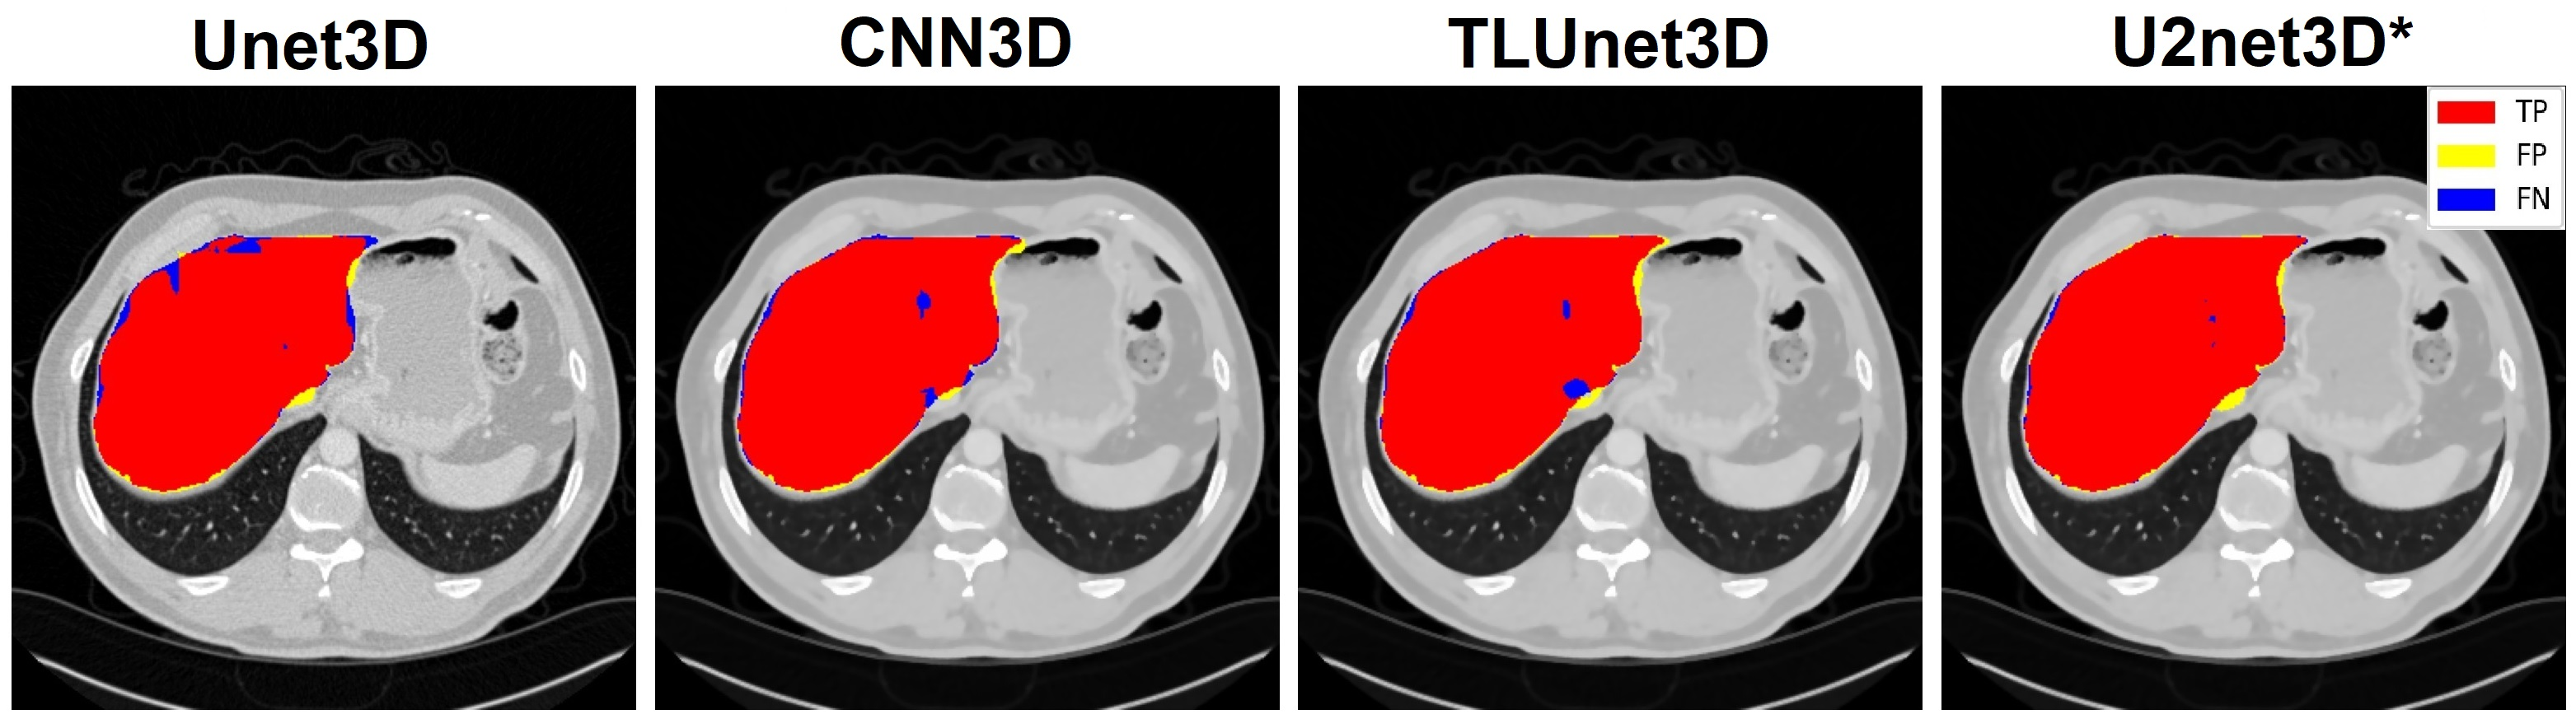
\includegraphics[width=\textwidth]{images/liver/U2Net3D/liver-result-legend.jpg}
    \caption{Kết quả dự đoán một mẫu dữ liệu trên tập Sliver07.}
    \label{fig:u2net3d-liver-result}
\end{figure}
\vspace{-5mm}
Hình \ref{fig:u2net3d-liver-result} minh họa kết quả dự đoán trên một lát cắt trên tập Sliver07 của các mô hình. Nhìn chung, các mô hình đều cho kết quả phân đoạn khá sát với thực tế, chỉ một vài phần nhỏ chưa phân đoạn được. Mô hình U2net3D* cho kết quả phần nền dự đoán sai (màu xanh) ít hơn các mô hình còn lại.
\subsection{Phân đoạn mạch máu}
Đối với bài toán phân đoạn mạch máu, mô hình đề xuất U2net3D* đã đạt được sự cải tiến lớn. Hệ số tương đồng (Dice) tăng 4\% (từ \textbf{ 56,29\%} lên đến \textbf{60.75\%}). Mặc dù độ chính xác có giảm bởi tỷ lệ dự đoán nhầm tăng nhưng độ phủ (Recall) cải thiện đáng kể.

\begin{table}[H]
    \renewcommand{\arraystretch}{1.1}
    \centering
    \begin{tabular}{c l c c c}
        \Xhline{2\arrayrulewidth}
        \multirow{2}{*}{\textbf{STT}} & \multirow{2}{*}{\textbf{Mô hình}} & \multicolumn{3}{c}{\textbf{Tập kiểm tra}} \\ \cline{3-5}
        & &  \textbf{Dice} & \textbf{Recall} & \textbf{Precision} \\ 
        \Xhline{2\arrayrulewidth}
        1   & Unet2D\cite{Unet}      & 41.17 & 60.05 & 31.32\\
        2   & Unet3D\cite{LV_LIVER}       & 56.29 & 44.27 & \textbf{73.97} \\
        3   & CNN3D\cite{LV_VESEL}        & 54.26 & 54.98 & 59.16 \\
        4   & U2net3D*     & \textbf{60.75} & \textbf{66.87} & 59.73 \\
        \Xhline{2\arrayrulewidth}
    \end{tabular}
    \caption{Kết quả phân đoạn mạch máu của các mô hình (\%).}
\end{table}

Để đánh giá một cách chi tiết các mẫu dữ liệu trong tập kiểm tra, chúng tôi đã tiến hành đánh giá trên từng bệnh nhân như sau. Mặc dù tập kiểm tra chỉ có 3 bệnh nhân tuy nhiên, trong quá trình huấn luyện mô hình chúng tôi không sử dụng toàn bộ 1 volume của 1 bệnh nhân để forward qua một lần mà sử dụng các khối sub-volume nhỏ hơn được sinh ra từ volume ban đầu. Do đó mặc dù chỉ chứa 3 bệnh nhân nhưng số lượng mẫu được lan truyền qua mạng cũng có số lượng đủ lớn (khoảng 350 sub-volume có kích thước 64$\times$96$\times$96) để đánh giá hiệu quả của mô hình. 
\begin{table}[H]
    \renewcommand{\arraystretch}{1.1}
    \centering
    \begin{tabular}{c l c c c}
        \Xhline{2\arrayrulewidth}
        \multirow{2}{*}{\textbf{STT}} & \multirow{2}{*}{\textbf{Bệnh nhân}} & \multicolumn{3}{c}{\textbf{Tập kiểm tra}} \\ \cline{3-5}
        & &  \textbf{Dice} & \textbf{Recall} & \textbf{Precision} \\ 
        \Xhline{2\arrayrulewidth}
        1   & Bệnh nhân số 1 & 50.73 & \textbf{82.85} & 36.55\\
        2   & Bệnh nhân số 6 & 62.52 & 65.66 & 59.76 \\
        3   & Bệnh nhân số 11 & \textbf{68.79} & 64.09 & \textbf{74.23} \\
        \Xhline{2\arrayrulewidth}
    \end{tabular}
    \caption{Kết quả phân đoạn mạch máu chi tiết các bệnh nhân trong tập kiểm tra(\%).}
    \label{tab:vessel-result-patient}
\end{table}

Dựa vào bảng \ref{tab:vessel-result-patient} có thể thấy được bệnh nhân số 6 và bệnh nhân số 11 cho kết quả rất tốt, hơn nữa 2 độ đo Recall và Precision khá tương đồng. Tuy nhiên khi đánh giá bệnh nhân số 0 thuộc trường hợp xấu nhất, điều này có thể giải thích được bởi việc thiếu dữ liệu huấn luyện. Nhắc lại quy trình chia dữ liệu được đề cập ở chương 4 bảng \ref{tab:training-set-vessel}, có thể thấy bệnh nhân số 1 thuộc nhóm dữ liệu có giá trị Hounsfield Unit trung bình cao nhất trong 3 nhóm. Đặc biệt hơn nhóm này chỉ có 2 bệnh nhân để đưa vào huấn luyện. Do đó có thể kết luận được việc tại sao bệnh nhân số 1 này lại đưa ra kết quả tệ nhất, bởi việc không đủ dữ liệu có thể đại diện cho mẫu này do đó mô hình vẫn chưa có khả năng dự đoán 1 cách chính xác nhất nếu rơi vào trường hợp này. Sau đây là histogram biễu diễn phân phối Hounsfield Unit của 3 bệnh nhân trong tập kiểm tra.

\begin{figure}[H]
    \centering
    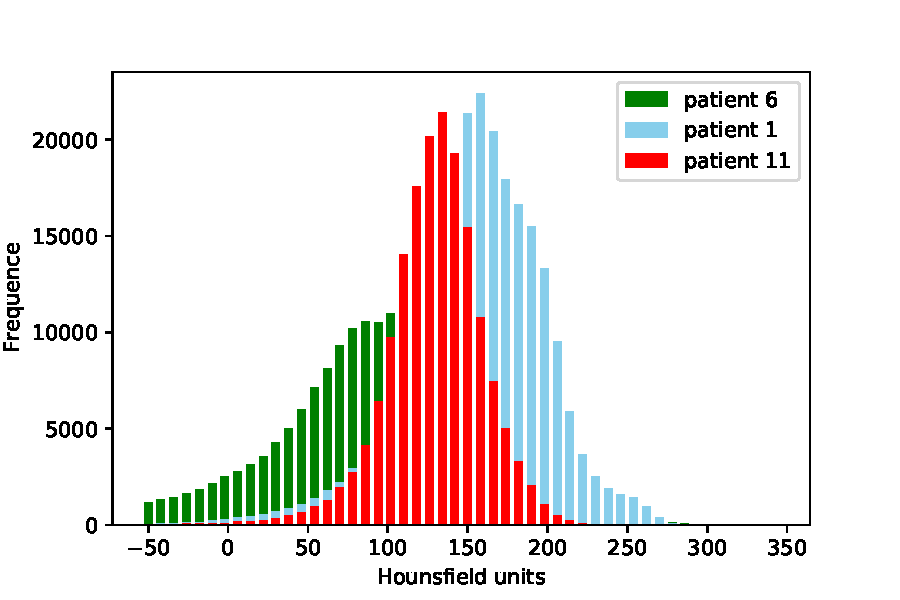
\includegraphics[width=.7\textwidth]{images/blood/test_hist.pdf}
    \caption{Phân phối Hounsfield Unit của các bệnh nhân trong tập kiểm tra.}
\end{figure}

Có thể thấy phân bố các giá trị hounsfield unit của bệnh nhân 1 phân bố ở vùng có giá trị cao hơn các bệnh nhân còn lại. Sau đây là kết quả trực quan của từng bệnh nhân:

\begin{figure}[H]
    \centering
    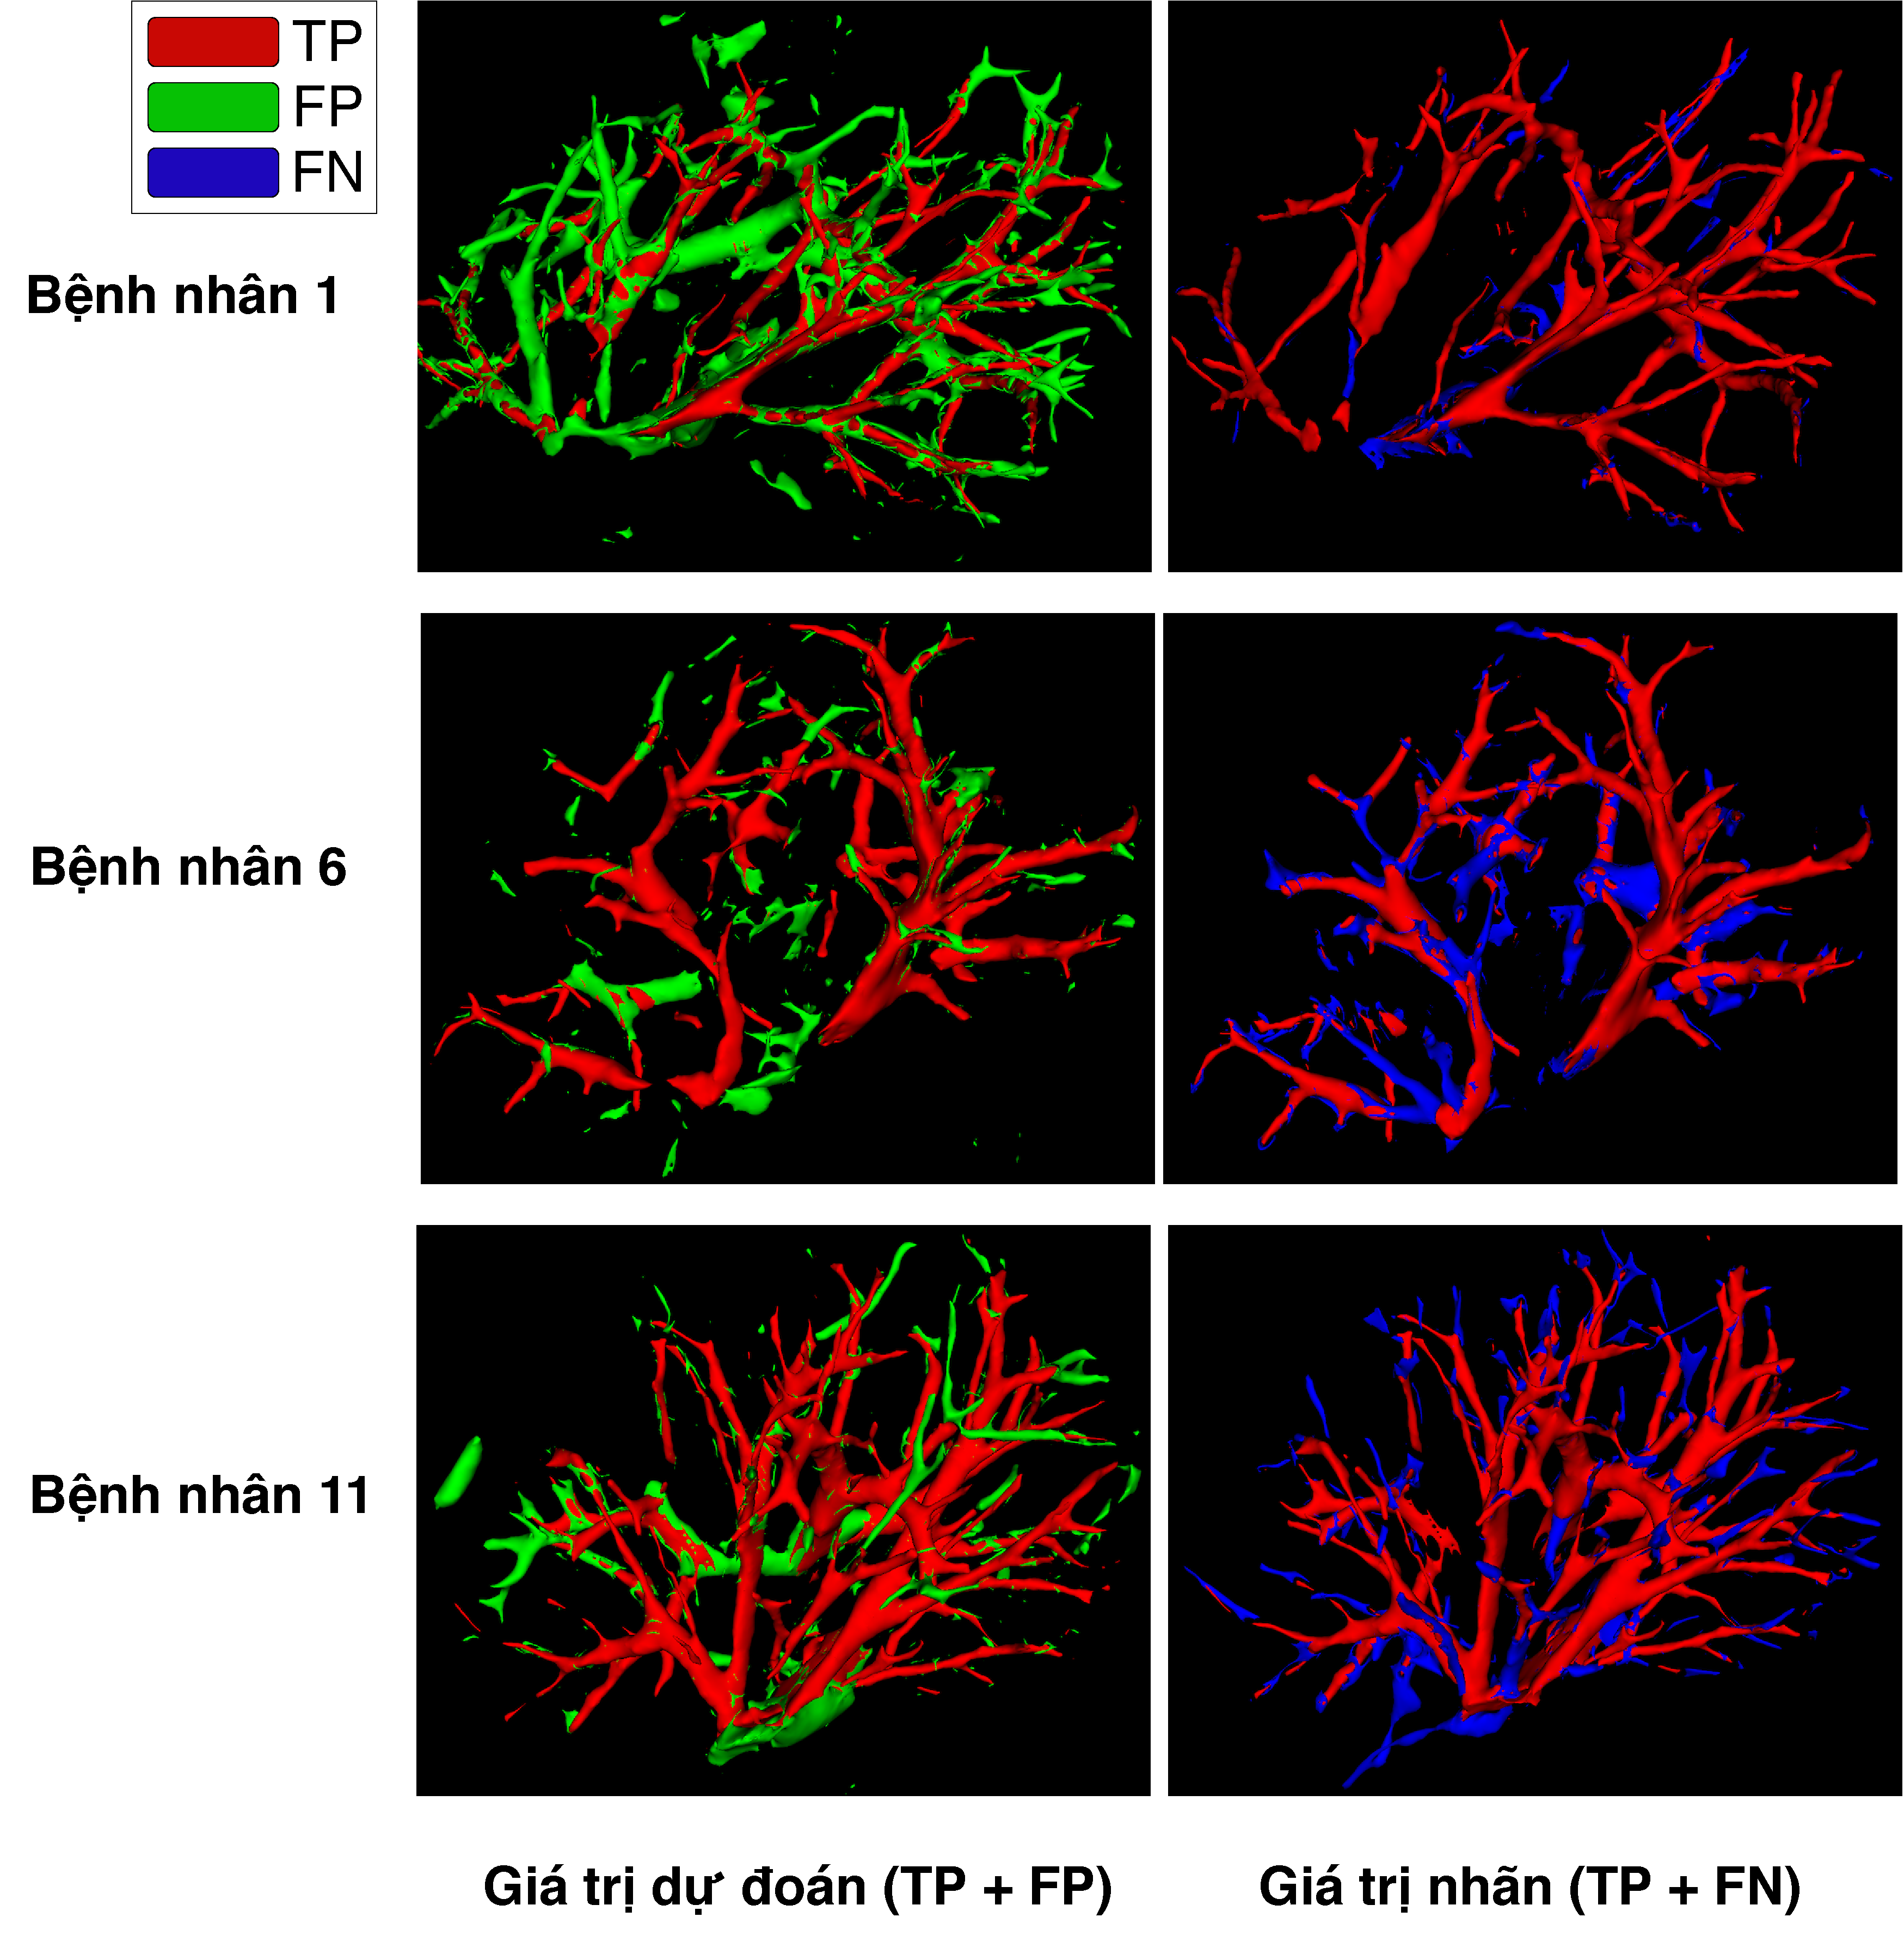
\includegraphics[width=\textwidth]{images/blood/3d_vessel.pdf}
    \caption{Kết quả trực quan hóa dưới dạng 3D của từng bệnh nhân.}
    \label{fig:3d-vessel}
\end{figure}

Dựa vào hình \ref{fig:3d-vessel} cho thấy được bệnh nhân 1 có kết quả dự đoán khá là nhiễu bởi mẫu này cho ra độ precision thấy, tuy nhiên độ recall lại cao nhất trong 3 bệnh nhân nên vùng màu xanh dương khá là ít. Trong khi đó 2 bệnh nhân còn lại cho ra kết quả khá tương đồng với mạch máu thật, ít bị nhiễu bởi False Positive hơn.
